

\documentclass{beamer}

\mode<presentation> {

\usetheme{Madrid}

}

\usepackage{graphicx} 
\usepackage{booktabs} 
\usepackage{tikz}

\title[Commutative S-rings]{Commutative S-rings Over Finite
  Groups} 

\author[Bruce Chiarelli]{Bruce Chiarelli \and Dr. Stephen Humphries} 
\institute[BYU]{Brigham Young University}
\date{March 15, 2014} 

\begin{document}
%%%%%%%%%%%%%%%%%%%%%%%%%%%%%

\begin{frame}
\titlepage 
\end{frame}

%%%%%%%%%%%%%%%%%%%%%%%%%%%%%

\begin{frame}
\frametitle{S-rings}
\begin{itemize}
\item Let $G$ be a finite group and $\mathbb{C}G$ be the complex group
  algebra over $G$.\pause
\item Let $\pi=(\Gamma_1,\Gamma_2,\ldots,\Gamma_n)$ be a partition of
  $G$. For each $\Gamma_i$, let
  $\overline{\Gamma_i}=\sum_{g\in\Gamma_i}g$.\pause
\item The $\Gamma_i$ will be called \textit{basic sets}.\pause
\begin{block}{Definition}
  The set $\{\overline{\Gamma_1}, \overline{\Gamma_2}
  ,\ldots,\overline{\Gamma_n}\}$ is a basis for a subring of
  $\mathbb{C}G$ called a \textit{Schur ring} (or \textit{S-ring}) if
  it has the following properties:
\begin{enumerate}
\item $\overline{\Gamma_1}=\mathrm{Id}_G$\pause
\item For each $\Gamma_i$, there exits some $\Gamma_i^{-1}\in\pi$ such
  that for every $g\in\Gamma_i$, $g^{-1}\in\Gamma_i^{-1}$.\pause
\item For each $\Gamma_i, \Gamma_j\in\pi$, there exist
  $a_k\in\mathbb{Z}$ such that $\overline{\Gamma_i}
  \overline{\Gamma_j}=\sum_{k=1}^{n}a_k\overline{\Gamma_k}$.
\end{enumerate}
\end{block}
\end{itemize}
\end{frame}

%%%%%%%%%%%%%%%%%%%%%%%%%%%%

\begin{frame}
\frametitle{Examples of S-rings}

\begin{block}{Extremes}
\begin{itemize}
\item For any group $G$, the \emph{trivial S-ring} has the basic sets\\
$\Gamma_1=\{1\}$\\ $\Gamma_2=G\backslash \{1\}$\pause
\item The entire group algebra $\mathbb{C}G$ is also an S-ring, given
  by the complete partition of the group. \pause
\end{itemize}
\end{block}

\begin{itemize}
\item In addition to the above, two further examples in $S_3$ are:
\end{itemize}

\begin{columns}
\column{.45\textwidth}
Conjugacy classes:
\begin{itemize}
\item $\Gamma_1=\{1\}$
\item $\Gamma_2=\{(1\,2), (1\,3), (2\,3)\}$
\item $\Gamma_3=\{(1\,2\,3),(1\,3\,2)\}$
\end{itemize}
\column{.45\textwidth}
\begin{itemize}
\item $\Gamma_1=\{1\}$
\item $\Gamma_2=\{(1\,2),(1\,3)\}$
\item $\Gamma_3=\{(2\,3)\}$
\item $\Gamma_4=\{(1\,2\,3),(1\,3\,2)\}$
\end{itemize}
\end{columns}
\end{frame}

%%%%%%%%%%%%%%%%%%%%%%%%%%%%%%

\begin{frame}
\frametitle{S-rings from partitions of transpositions}
\begin{itemize}
\item When have we chosen a partition such that the S-ring is commutative?\pause
\item Let $G=S_n$ and consider a partition of the transpositions $T = 
  T_1 \cup T_2 \cup \ldots \cup T_r $\pause
\item By exponentiation, we can deduce the other basic sets
  by comparing coefficients.\pause
\item Example (in $S_4$): Let $\overline{T_1} = (1\,2)+(1\,3)+(1\,4)$ \pause
\item Then $ \overline{T_1}^3 = 2\left[(3\,4) +
    (2\,3) + (2\,4)\right] + 5\left[ (1\,2) + (1\,3) + (1\,4)\right] +
  \cdots$\pause
\item $\overline{T_1}^4 = 15\mathrm{Id} + 3\left[(2\,3\,4) + (2\,4\,3)\right] +
  8\left[ (1\,2\,3) + (1\,3\,2) + (1\,2\,4) + (1\,4\,2) + (1\,3\,4) +
    (1\,4\,3)\right]+\cdots$
\end{itemize}
\end{frame}

\begin{frame}
\frametitle{Combinatorial properties}
\begin{itemize}
\item When does a partition of the transpositions give basic sets
  $T_1, T_2,\ldots T_r$ such that $\overline{T_i}$ and
  $\overline{T_j}$ commute?\pause
\item There is a natural coloring of the edges of the complete graph
  $K_n$ corresponding to $T$. \pause For example, in $S_4$:
\vspace{.5cm}
\begin{columns}
\column{.4\textwidth}
\begin{figure}
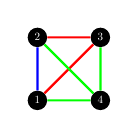
\begin{tikzpicture}
  [scale=.8,auto=left,every node/.style={circle,color=white,fill=black,scale=.4}]
  \node (n1) at (1,1) {1};
  \node (n2) at (1,2) {2};
  \node (n3) at (2,2) {3};
  \node (n4) at (2,1) {4};

  \draw[thick,blue] (n1) -- (n2);

  \draw[thick,red] (n1) -- (n3);
  \draw[thick,red] (n2) -- (n3);

  \draw[thick,green] (n1) -- (n4);
  \draw[thick,green] (n2) -- (n4);
  \draw[thick,green] (n3) -- (n4);
\end{tikzpicture}
\end{figure}
\column{.5\textwidth}
$\{\textcolor{blue}{(1\,2)},$\\
$\textcolor{red}{[(1\,3)+(2\,3)]},$\\ 
$\textcolor{green}{[(1\,4)+(2\,4)+(3\,4)]}\}$
\end{columns}
\vspace{.5cm}\pause
\item What conditions does the corresponding graph coloring satisfy if
  $\overline{T_i}\,\overline{T_j} = \overline{T_j}\,\overline{T_i}$?
\end{itemize}
\end{frame}

%%%%%%%%%%%%%%%%%%%%%%%%%%%%%

\begin{frame}
\frametitle{Constrained colorings}
\begin{itemize}
\item Trivial cases: $(i\,j)(k\,l)$, $(i\,j)(i\,j)$ are
  summands.
\begin{itemize}
\item The edges $(i, j)$ and $(k, l)$ share no vertices.\pause
\end{itemize}
\item Every 3-cycle can be decomposed into transpositions in three
  ways: $(i\,j\,k)=(i\,j)(j\,k)=(i\,k)(i\,j)=(j\,k)(i\,k)$\pause
\item Let $C$ and $D$ be disjoint sets of transpositions in $S_n$. If
  $\overline{C}\,\overline{D} = \overline{D}\,\overline{C}$ and
  $(i\,j)\in C$ and $(j\,k)\in D$, then $(i\,j\,k)$ is a summand of
  both $\overline{C}\,\overline{D}$ and
  $\overline{D}\,\overline{C}$. Checking the possibilities, $(i\,k)$
  must be in $C$ or $D$.\pause
\begin{itemize}
\item \color<6->{red}{On the corresponding graph, this means that the triangle with
  vertices $i,j,k$ is two-colored.}\pause
\end{itemize}
\item Now assume that $(i\,j), (i\,k)\in C$ and $(j\,k)\in D$. Then
  $(i\,j\,k)$ is a summand of $\overline{C}\,\overline{D}$, and occurs
  only once. Then since $(j\,k)(i\,k) = (i\,j\,k)$, the summand occurs
  in $\overline{D}\,\overline{C}$ as well. A similar argument holds if
  $(i\,k)\in D$.
\end{itemize}
\end{frame}

%%%%%%%%%%%%%%%%%%%%%%%%%%%%

\begin{frame}
\frametitle{Gallai colorings}
\begin{block}{Definition}
An edge coloring of the complete graph $K_n$ is said to be \emph{Gallai} if no
triangle in the graph is tri-colored. \pause
\end{block}
\begin{columns}
\column{.4\textwidth}
Examples:
\begin{figure}
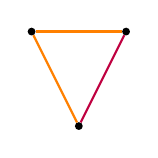
\begin{tikzpicture}
  [scale=.6,auto=left,every node/.style={circle,color=white,fill=black,scale=.3}]
  \node (n1) at (1,4) {};
  \node (n2) at (2,2)  {};
  \node (n3) at (3,4)  {};

  \draw[thick,orange] (n1) -- (n2);
  \draw[thick,purple] (n2) -- (n3);
  \draw[thick,orange] (n3) -- (n1);

\end{tikzpicture}
\end{figure}

\begin{figure}
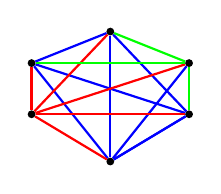
\begin{tikzpicture}
  [scale=.5,auto=left,every node/.style={circle,color=white,fill=black,scale=.3}]
  \node (n1) at (2,.8) {};
  \node (n2) at (4,2) {};
  \node (n3) at (4,3.3) {};
  \node (n4) at (2,4.1) {};
  \node (n5) at (0,3.3) {};
  \node (n6) at (0,2) {};

  \draw[thick,blue] (n1) -- (n2);
  \draw[thick,blue] (n1) -- (n2);
  \draw[thick,blue] (n1) -- (n3);
  \draw[thick,blue] (n1) -- (n4);
  \draw[thick,blue] (n1) -- (n5);
  \draw[thick,blue] (n2) -- (n4);
  \draw[thick,blue] (n2) -- (n5);
  \draw[thick,blue] (n4) -- (n5);

  \draw[thick,red] (n6) -- (n1);
  \draw[thick,red] (n6) -- (n2);
  \draw[thick,red] (n6) -- (n3);
  \draw[thick,red] (n6) -- (n4);
  \draw[thick,red] (n6) -- (n5);

  \draw[thick,green] (n2) -- (n3);
  \draw[thick,green] (n3) -- (n4);
  \draw[thick,green] (n3) -- (n5);
\end{tikzpicture}
\end{figure}\pause
\column{.4\textwidth}
Non-examples:
\begin{figure}
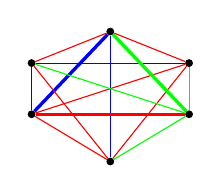
\begin{tikzpicture}
  [scale=.5,auto=left,every node/.style={circle,color=white,fill=black,scale=.3}]
  \node (n1) at (2,.8) {};
  \node (n2) at (4,2) {};
  \node (n3) at (4,3.3) {};
  \node (n4) at (2,4.1) {};
  \node (n5) at (0,3.3) {};
  \node (n6) at (0,2) {};

  \draw[blue] (n3) -- (n5);
  \draw[very thick,blue] (n6) -- (n4);
  \draw[blue] (n6) -- (n5);
  \draw[blue] (n1) -- (n4);

  \draw[red] (n1) -- (n6);
  \draw[red] (n1) -- (n5);
  \draw[red] (n1) -- (n3);
  \draw[very thick,red] (n2) -- (n6);
  \draw[red] (n3) -- (n4);
  \draw[red] (n3) -- (n6);
  \draw[red] (n4) -- (n5);

  \draw[green] (n2) -- (n1);
  \draw[green] (n2) -- (n5);
  \draw[very thick,green] (n2) -- (n4);
  \draw[green] (n2) -- (n3);
\end{tikzpicture}
\end{figure}

\begin{figure}
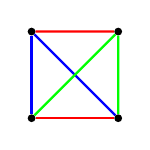
\begin{tikzpicture}
  [scale=1.1,auto=left,every node/.style={circle,color=white,fill=black,scale=.3}]
  \node (n1) at (1,1) {};
  \node (n2) at (1,2) {};
  \node (n3) at (2,2) {};
  \node (n4) at (2,1) {};


  \draw[thick,blue] (n1) -- (n2);
  \draw[thick,blue] (n2) -- (n4);

  \draw[thick,red] (n1) -- (n4);
  \draw[thick,red] (n2) -- (n3);

  \draw[thick,green] (n1) -- (n3);
  \draw[thick,green] (n3) -- (n4);
\end{tikzpicture}
\end{figure}

\end{columns}
\end{frame}

%%%%%%%%%%%%%%%%%%%%%%%%%%%%%%%%%

\begin{frame}
\frametitle{Commutativity of sums of transpositions}
\begin{block}{Theorem}
A partition of transpositions in $S_n$ gives commuting elements of
$\mathbb{C}S_n$ if and only if the edge coloring of the corresponding graph is Gallai.\pause
\end{block}
\vspace{.4cm}
\begin{columns}
\column{.4\textwidth}
\onslide<2->{
\begin{figure}
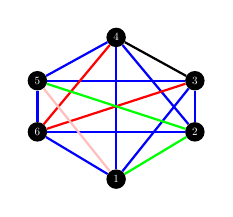
\begin{tikzpicture}
  [scale=.5,auto=left,every node/.style={circle,color=white,fill=black,scale=.4}]
  \node (n1) at (2,.8) {1};
  \node (n2) at (4,2) {2};
  \node (n3) at (4,3.3) {3};
  \node (n4) at (2,4.4) {4};
  \node (n5) at (0,3.3) {5};
  \node (n6) at (0,2) {6};

  \draw[thick,blue] (n1) -- (n3);
  \draw[thick,blue] (n1) -- (n4);
  \draw[thick,blue] (n1) -- (n6);
  \draw[thick,blue] (n2) -- (n3);
  \draw[thick,blue] (n2) -- (n6);
  \draw[thick,blue] (n2) -- (n4);
  \draw[thick,blue] (n3) -- (n5);
  \draw[thick,blue] (n4) -- (n5);
  \draw[thick,blue] (n5) -- (n6);

  \draw[thick,red] (n3) -- (n6);
  \draw[thick,red] (n4) -- (n6);

  \draw[thick,green] (n1) -- (n2);
  \draw[thick,green] (n2) -- (n5);

  \draw[thick,pink] (n1) -- (n5);

  \draw[thick,black] (n3) -- (n4);
\end{tikzpicture}
\end{figure}}
\onslide<2->{
\column{.5\textwidth}
$\{\textcolor{blue}{[(1\,3)+(1\,4)+(1\,6)+(2\,3)}$\\
$\textcolor{blue}{+(2\,4)+(2\,6)+(3\,5)+(4\,5)+(5\,6)]},$\\
$\textcolor{red}{[(3\,6)+(4\,6)]},$\\ 
$\textcolor{green}{[(1\,2)+(2\,5)],}$\\
$\textcolor{pink}{(1\,5)},$\\
$\textcolor{black}{(3\,4)}\}$}
\end{columns}\pause
\begin{itemize}
\item Maximal commuting partitions have $n-1$ parts (colors).
\end{itemize}
\end{frame}

%%%%%%%%%%%%%%%%%%%%%%%%%%%%

\begin{frame}
\frametitle{Maximal commutative partitions}
\begin{itemize}
\item Every Gallai-colored complete graph has a color whose edges span all the
  vertices. \pause
\item If the coloring has the maximum $n-1$ colors, removing all edges
  of the spanning color will result in exactly two connected components. \pause
\item By recursively splitting the graph in this way, we obtain a
  rooted binary tree where each caret corresponds to a color. For
  example:\pause
\begin{columns}
\column{.33\textwidth}
\begin{figure}
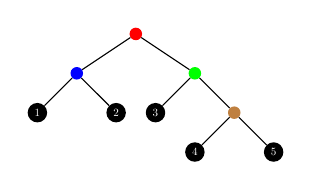
\begin{tikzpicture}
  [scale=.5,auto=left,every node/.style={circle,color=white,fill=black,scale=.4}]
\onslide<7->{  \node (n1) at (0,1) {1};
  \node (n2) at (2,1) {2};}
\onslide<7->{  \node (n3) at (3,1) {3};}
\onslide<8->{  \node (n4) at (4,0) {4};
  \node (n5) at (6,0) {5};}

\onslide<7->{  \node [brown,scale=1.2] (n6) at (5,1) {};}
\onslide<6->{  \node [green,scale=1.2] (n7) at (4,2) {};
  \node [blue,scale=1.2] (n8) at (1,2) {};}
\onslide<5->{  \node [red,scale=1.2] (n9) at (2.5,3) {};}

\onslide<7->{  \draw (n1) -- (n8);
  \draw (n2) -- (n8);}
\onslide<6->{  \draw (n8) -- (n9);
  \draw (n9) -- (n7);}
\onslide<7->{  \draw (n7) -- (n3);}
\onslide<7->{  \draw (n7) -- (n6);}
\onslide<8->{  \draw (n6) -- (n5);
  \draw (n6) -- (n4);}

\end{tikzpicture}
\end{figure}
\column{.33\textwidth}
\begin{figure}
\begin{tikzpicture}
  [scale=.5,auto=left,every node/.style={circle,color=white,fill=black,scale=.4}]
  \node (n1) at (3,3) {1};
  \node (n2) at (1,2) {2};
  \node (n3) at (5,2) {3};
  \node (n4) at (2,0) {4};
  \node (n5) at (4,0) {5};

\only<4-5,8->{  \draw [blue,thick] (n1) -- (n2);}
\only<4,8->{  \draw [red,thick] (n2) -- (n3);

  \draw [red,thick] (n5) -- (n1);

  \draw [red,thick] (n1) -- (n3);
  \draw [red,thick] (n1) -- (n4);
  \draw [red,thick] (n2) -- (n4);
  \draw [red,thick] (n2) -- (n5);}

\only<4-5,8->{  \draw [green,thick] (n3) -- (n4);
  \draw [green,thick] (n3) -- (n5);}
\only<4-6,8->{  \draw [brown,thick] (n4) -- (n5);}


\end{tikzpicture}
\end{figure}\pause
\column{.33\textwidth}
\onslide<9->{
$\{\textcolor{red}{(1\,3)+(1\,4)+(1\,5)}$\\ %% LaTeX complains about newlines inside $...$
$\textcolor{red}{+(2\,3)+(2\,4)+(2\,5)}$,\\
$\textcolor{green}{(3\,4)+(3\,5)}, \textcolor{blue}{(1\,2)}$,\\
$\textcolor{brown}{(4\,5)}\}$
}
\end{columns}
\onslide<10->{
\item The number of isomorphism classes of rooted binary trees is
  given by the Wedderburn-Etherington numbers: 1, 1, 2, 3, 6, 11, 23,
  \ldots}
\end{itemize}
\end{frame}

%%%%%%%%%%%%%%%%%%%%%%

\begin{frame}
\Huge{\centerline{Thank you!}}
\end{frame}

\end{document} 